%% Section 4: The RevTrace System. Three-element pattern per module:
%% motivation / mechanism / evidence hook. (outline v2 sec.3.4)

RevTrace implements DGFT as a transaction runtime: per-family adapters, a
versioned ledger, and a stratified certification layer
(Figure~\ref{fig:arch}).

\begin{figure*}[t]
  \centering
  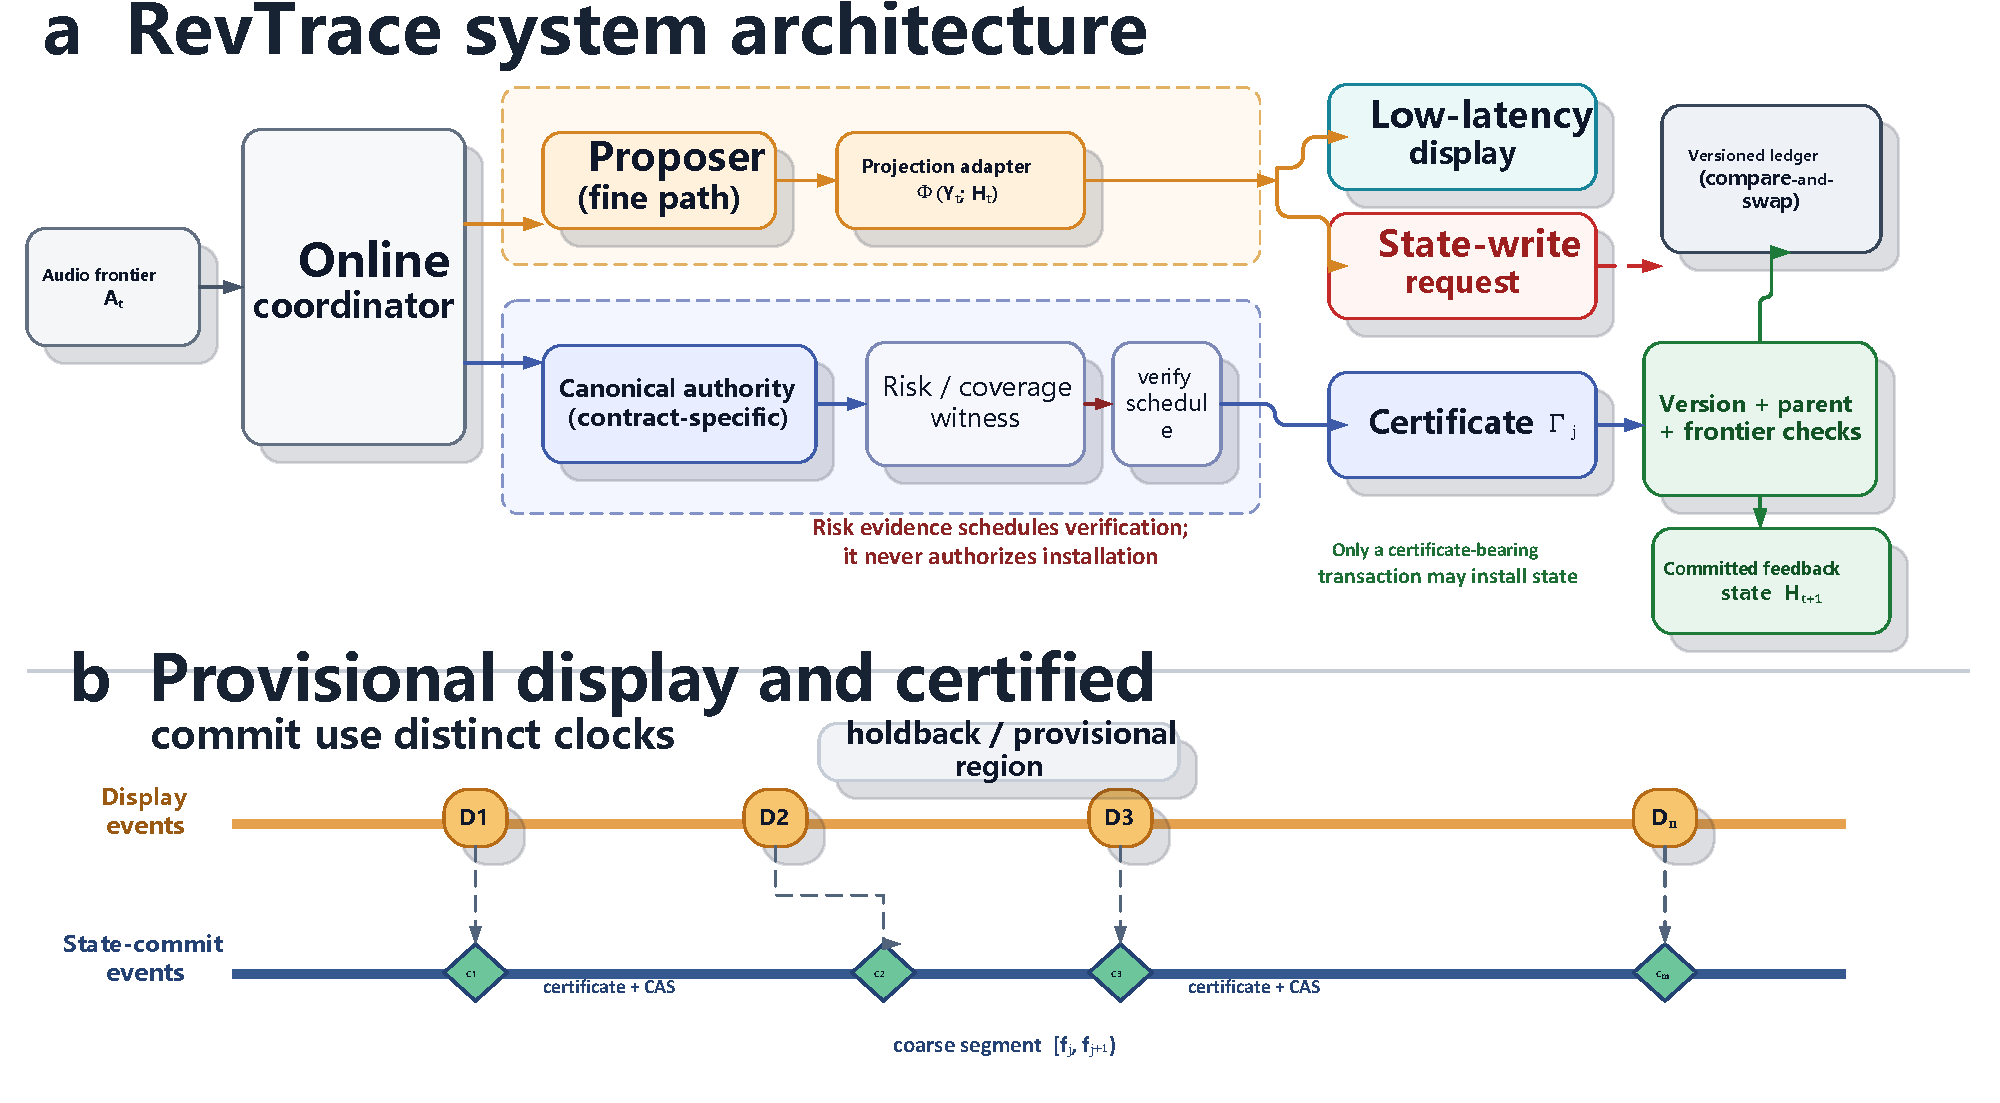
\includegraphics[width=\textwidth]{figures/f2_architecture_visio.pdf}
  \caption{RevTrace architecture (top) and the DGFT commit timeline (bottom).
  Provisional display and state write are separate permissions; only a
  certificate-bearing transaction whose parent version and frontier checks
  pass may advance committed state. Risk and coverage evidence may schedule
  verification but cannot authorize installation.}
  \label{fig:arch}
\end{figure*}

\subsection{Architecture-specific adapters}\label{sec:sys:adapters}

\emph{Motivation.} The safety proofs of Section~\ref{sec:dgft} require only
three interfaces; everything family-specific must stay out of the protocol.
\emph{Mechanism.} Each family provides (i) a state-projection adapter
computing $\proj(\out_t;H_t)$ (Qwen rollback prefix; Whisper
previous-text prompt), (ii) an authority adapter executing the canonical
path (FP16 singleton for SG; FP32 batched for Coarse/Hybrid), and
(iii) an evidence adapter collecting risk signals (margins, directional
coverage, repetition) for the certification layer.
\emph{Evidence hook.} H4 (Section~\ref{sec:eval}) runs the identical
runtime over both families through these adapters.

\subsection{Certificate and versioned ledger}\label{sec:sys:ledger}

\emph{Motivation.} R2/R3 require detecting staleness and frontier
discontinuity at commit time. \emph{Mechanism.} A compare-and-swap-style
ledger stores committed state versions; every commit tuple
$\commit_j$ (Definition~\ref{def:commit}) is checked against session,
contract epoch, policy, and state-version fences before installation, and
each accepted commit consumes its certificate exactly once.
\emph{Evidence hook.} H2: exhaustive transaction validation reports every
install attempt against these fences (320 Qwen events; 1{,}048 Whisper
commits; zero violations).

\subsection{Directional coverage and selective fine replay}\label{sec:sys:coverage}

\emph{Motivation.} A coarse authority segment must be witnessed against the
fine proposals it replaces; replaying everything would forfeit the point of
coarse authority. \emph{Mechanism.} The coverage witness records, in Latin
and CJK units, which fine-region outputs the coarse certificate accounts
for; uncovered regions are queued for fine replay. Hybrid adds
risk-triggered replay at fraction $r$, trading cost for quality
(Eq.~\eqref{eq:cost-dgft}). \emph{Evidence hook.} H3 ablates $r=0$
(Coarse) against $r>0$ (Hybrid) on the same workload.

\subsection{Stratified certification}\label{sec:sys:cert}

Four strata, each with a non-transferable scope
(Figure~\ref{fig:cert}):
(i) \emph{SG numerical risk}: randomized audits of the singleton authority
with anytime-valid (UCB) bounds, scoped to the SG adapter
path~\cite{howard2021confidence,ramdas2023savi};
(ii) \emph{authority implementation}: contract-scoped FP32 preflight
invariance checks (batch repeat, batch-vs-singleton), fail-closed;
(iii) \emph{transaction integrity}: exhaustive online validation of
certificates, versions, and frontier continuity;
(iv) \emph{semantic quality}: independent per-family references.
A risk signal from any stratum may schedule verification but never authorize
installation (R4).

\begin{figure}[t]
  \centering
  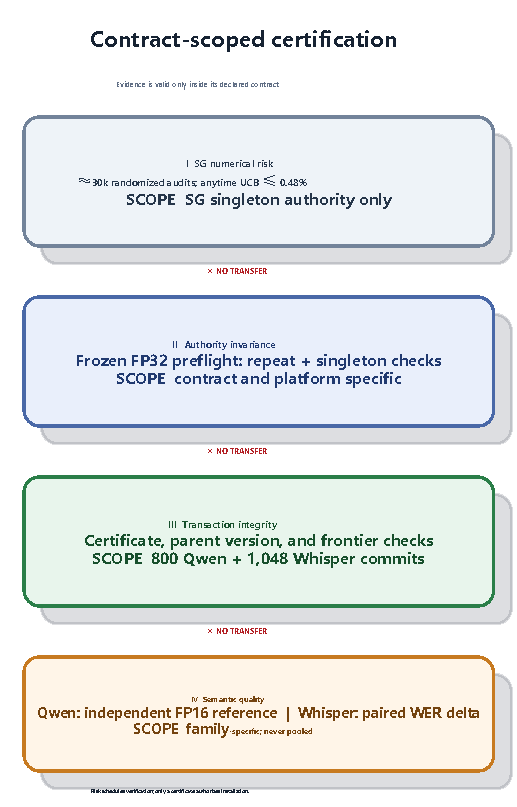
\includegraphics[width=\columnwidth]{figures/f3_certification_visio.pdf}
  \caption{Stratified, contract-scoped certification. Each rung yields exactly one
  scope-limited guarantee; no rung's evidence authorizes another's
  installation decisions.}
  \label{fig:cert}
\end{figure}

\subsection{Online coordinator}\label{sec:sys:coord}

The coordinator schedules the proposer and authority lanes on separate
GPUs (Eq.~\eqref{eq:cost-service}), invalidates stale descendants
(Corollary~\ref{cor:stale}), closes terminal frontiers at session end, and
performs rollback/rebase when a commit supersedes displayed provisional
state.
